\section{Wall adsorption and local roughness}
\label{sec:swall}

A wall between all-alive and all-dead regions develops an active layer even when
the bulk active phase is metastable. Below the measured front reversal the
layer approaches a slowly varying thickness; above it the two edges move apart as active--absorbing
fronts. This geometry probes the competition among all three phases without
preparing an active region initially.

We measure the number $I=L_y\iota/2$ of interface sites per unit wall length and subtract
the $q=0$ value $I_0\simeq8.7$ to obtain the excess adsorption
$\Gamma=I-I_0$. Earlier measurements give an increase from about 10 at
$q=0.03672$ to about 109 at $q=0.0456705$. This increase is reproduced
across wall lengths $L_x=256$--4096 and transverse sizes $L_y=1024$--4096
(Fig.~\ref{fig:wall}). Runs last $10^6$--$3\times10^6$ steps.
For the late-window estimates we time-average each run over
$t\ge\max(3\times10^5,T/2)$ and then average independent runs.
Some walls wander far enough to consume one of the absorbing slabs. We terminate
their averaging windows before the live fraction leaves $[0.3,0.7]$, record
these truncations, and use the larger transverse boxes for the closest points.
The seven-point legacy fit below contains three truncated run windows and
omits one run with no usable window. Its two $L_y=4096$ points use the
available $L_y=1024$ baseline. The uncertainty of each shared $q=0$ baseline
is retained in the fit covariance; these legacy fits are conditional on the
stated geometry windows and baseline choices.

The increase of $\Gamma$ is robust, but a pure power law is sensitive to the
coexistence point and to corrections to scaling. With $q^*=0.04594$ and
$\delta=1-q/q^*$, fitting $\Gamma=A\delta^{-\psi}$ to the seven
$L_x=1024$, $L_y\ge2048$ points gives an effective $\psi=0.524$.
The fit is inadequate within the run-to-run errors: $\chi^2=74.7$ for five
degrees of freedom. The equally parameterized form
$\Gamma=A\delta^{-1/3}+B$ instead gives $A=20.28$, $B=-27.43$, and
$\chi^2=10.53$ for five degrees of freedom. Both fits minimize residuals in
adsorption units. Varying $q^*$ over $[0.04592,0.04596]$ moves the effective
pure-power slope from 0.506 to 0.541 and the offset-form $\chi^2$ from
3.74 to 27.03. An additive correction therefore changes the interpretation
of the apparent slope, while its fit quality remains reference dependent.
These legacy data do not establish an asymptotic exponent.

\begin{figure*}
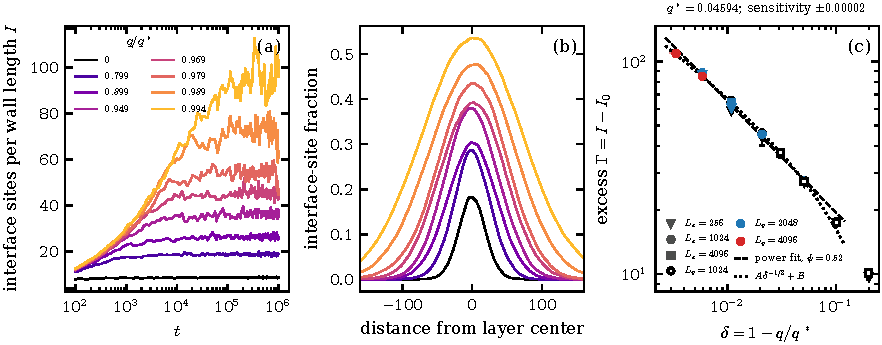
\includegraphics[width=\textwidth]{figs/fig_wall05}
\caption{Wetting at $p=1/2$, referenced to $q^*=0.04594$.
(a) Interface sites per unit wall length against time for $L_x=L_y=1024$
(four seeds per curve). (b) Interface-site fraction across the layer, centered
on its interface-weighted mean row before averaging late records.
(c) Excess adsorption for several box sizes (two to four seeds per point);
vertical bars show standard errors over runs including baseline uncertainty.
Horizontal bars on the fit points show the effect of varying $q^*$ by
$\pm0.00002$, a systematic sensitivity range. The dashed pure-power fit and
dotted $A\delta^{-1/3}+B$ fit use the same seven points with $L_x=1024$,
$L_y\ge2048$ and $\delta\le0.1$. The offset reduces the residuals, but neither fit determines the
asymptotic law.}
\label{fig:wall}
\end{figure*}

The extended test uses $L_y=8192$, wall lengths $L_x=4096$ and 16384,
and four independent $10^7$-step runs at each of three closer probabilities
(Fig.~\ref{M-fig:gpu_wetting}). Every ensemble is complete and retains the
full $5\times10^6$--$10^7$ averaging window, with a matched-size
$q=0$ baseline from two $2\times10^6$-step runs. All wall-separation
and global-density geometry checks pass. At $L_x=16384$, the excess
adsorptions are 133.27, 166.15, and 190.86 for $q=0.04584$, 0.04588,
and 0.04590. The corresponding $L_x=4096$ values are 134.80, 168.37,
and 199.90. At the closest probability, the larger system has about
4.5\% less adsorption; the run-bootstrap interval for this size difference
excludes zero. Its adsorption also declines by about 0.6\% between the
two halves of the late window, a small late-window change observed in all four runs.
These data extend the observed thickening while exposing finite-size
and finite-time corrections.

The new points test predictions from the earlier fits. At each fixed
front-derived reference, both candidate forms are fitted only to the
seven legacy points; their parameter uncertainty and shared-baseline
covariance are propagated to the predictions. Agreement at one new
probability does not imply a joint description of all three. The
extended measurements show discrepancies beyond their sampling errors
from the legacy extrapolations, together with the size and time effects
above. The analysis therefore does not assign an asymptotic wetting
exponent or treat either two-parameter extrapolation as a converged law.



The observed adsorption increase motivates a complete-wetting interpretation: near
coexistence an absorbing--absorbing interface separates into two
absorbing--active interfaces. Active boundary layers also occur between
defensive alliances~\cite{szabo2007}. In equilibrium, the interface between two
ordered phases can be wetted by the disordered phase at a first-order Potts
transition~\cite{selke1983,carlon1999}; fluctuating short-range interfaces in
two dimensions give the exponent $1/3$~\cite{lipowsky1983,fisher1984,carlon1999}.
Nonequilibrium wetting has also been studied with a bounded
Kardar--Parisi--Zhang interface~\cite{hinrichsen1997wet,munoz1998,delossantos2003}.
Here the layer is bounded by two fluctuating active--absorbing fronts.

The film edges show short-distance height-difference correlations close to
$\langle[h(x+r)-h(x)]^2\rangle\propto r$. Log--log fits over the recorded
separations $2\le r\le50$ give effective roughness exponents
$\zeta=0.468$, $0.499$, and $0.502$ for $L_x=256$, 1024, and 4096,
respectively. The local layer thickness has a broad distribution
(Fig.~\ref{fig:rough}). These finite-distance measurements motivate a
fluctuating-interface description, while the asymptotic exponent and
large-distance interaction remain unresolved.

\begin{figure*}
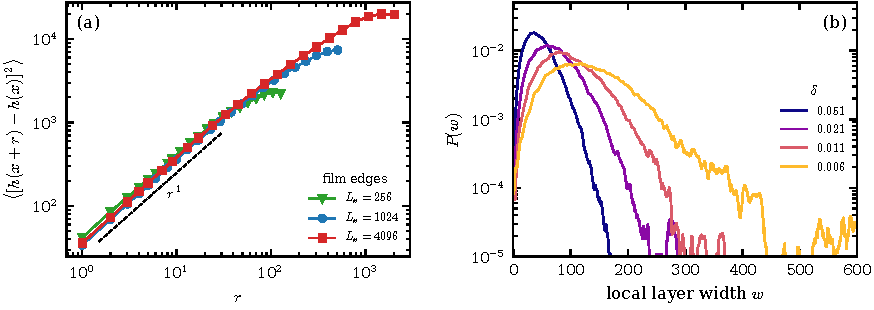
\includegraphics[width=\textwidth]{figs/fig_rough}
\caption{Edges of the wetting film at $p=\alpha=1/2$, from configurations
stored every $10^5$ steps for $t\ge10^5$, with $L_y=2048$.
(a) Height-difference correlation of both physical film edges at
$q=0.045441$, averaged equally over independent runs. The wall lengths
$L_x=256$, 1024, and 4096 have four, four, and two runs, respectively.
The dashed line shows $\propto r$, corresponding to $\zeta=1/2$.
(b) Local thickness distributions for $L_x=1024$ at $q=0.043605$,
0.044982, 0.045441, and 0.0456705. The legend gives
$\delta=1-q/q^*$ using $q^*=0.04594$. Curves show a five-bin moving
average of the run-averaged histograms.}
\label{fig:rough}
\end{figure*}

%=====================================================================================
